\documentclass[11pt]{book}
\usepackage[margin=1.2in]{geometry}
\usepackage[toc,page]{appendix}
\usepackage{graphicx}
\usepackage{natbib}
\usepackage{lipsum}
\usepackage{caption}
\usepackage[T1]{fontenc}
\usepackage{titlesec, blindtext, color}
\usepackage{xcolor,tikz}
\usepackage{caption}
\usepackage{subcaption}
\usetikzlibrary{patterns}
\usetikzlibrary{decorations.markings}
\usetikzlibrary{decorations.pathmorphing}
% \usepackage{amsmath,amssymb,amsthm,mathrsfs,amsfonts,xfrac,pifont,bbold,physics}
\usepackage[utf8]{inputenc}
\usepackage{amsthm}
\usepackage{pgfplots}
\usepackage[breakable, theorems, skins]{tcolorbox}
\usepackage[colorlinks = true,
            linkcolor = red,
            urlcolor  = blue,
            citecolor = red,
            anchorcolor = red]{hyperref}
\usepackage{enumitem}
\usepackage{TemplateMatma}
\usepackage{TemplateNotatkiPE}

\newcommand{\cmark}{\ding{51}}
\newcommand{\xmark}{\ding{55}}

\tikzset{
    partial ellipse/.style args={#1:#2:#3}{
        insert path={+ (#1:#3) arc (#1:#2:#3)}
    }
}



% -------------------------------------------------------------------
% Theorem Styles
% -------------------------------------------------------------------

\theoremstyle{definition} % Define theorem styles here based on the definition style (used for definitions and examples)
\newtheorem*{definition}{Definition}

\theoremstyle{plain} % Define theorem styles here based on the plain style (used for theorems, lemmas, propositions)
\newtheorem{theorem}{Theorem}[section]
\newtheorem{axiom}{Axiom}
\newtheorem{corollary}[theorem]{Corollary}
\newtheorem{lemma}[theorem]{Lemma}
\newtheorem{proposition}[theorem]{Proposition}
\newtheorem{postulate}{Postulate}

\theoremstyle{remark} % Define theorem styles here based on the remark style (used for remarks and notes)
\newtheorem*{solution}{Solution}


\newtheoremstyle{underline}% name
{}        % Space above, empty = `usual value'
{}              % Space below
{}              % Body font
{}    % Indent amount (empty = no indent, \parindent = para indent)
{}              % Thm head font
{.}             % Punctuation after thm head
{1.5mm}         % Space after thm head: \newline = linebreak
{{\underline{\textit{\thmname{#1}\thmnumber{ #2}}~\thmnote{(#3)}\unskip}}}  % Thm head spec

\theoremstyle{underline}

\newtheorem{remark}[theorem]{Remark}
\newtheorem{example}[theorem]{Example}
\newtheorem{claim}[theorem]{Claim}
\newtheorem{exercise}[theorem]{Exercise}
\newtheorem*{terminology}{Terminology}
\newtheorem*{notation}{Notation}
\newtheorem*{convention}{Convention}



% -------------------------------------------------------------------
% Chapter Headings
% -------------------------------------------------------------------

\setcounter{chapter}{0}

\makeatletter
\renewcommand{\@chapapp}{Lecture}
\makeatother
\definecolor{lightergray}{rgb}{0.9,0.9,0.9}

\usepackage{titlesec}
\titleformat{\section}{\large\bfseries\raggedright}{}{0em}{\colorsection}[\titlerule]
\titleformat{name=\section,numberless}{\large\scshape\bfseries\raggedright}{}{0em}{\colorsectionnonumber}[\titlerule]

\titleformat{\subsection}{\bfseries\raggedright}{}{0em}{\colorsubsection}
\titleformat{name=\subsection,numberless}{\bfseries\raggedright}{}{0em}{\colorsubsectionnonumber}

\newcommand{\colorsection}[1]{%
    \colorbox{lightergray}{\parbox{\dimexpr\textwidth-2\fboxsep}{\thesection\ \ #1}}}
\newcommand{\colorsectionnonumber}[1]{%
    \colorbox{lightergray}{\parbox{\dimexpr\textwidth-2\fboxsep}{#1}}}
    
\newcommand{\colorsubsection}[1]{%
    \colorbox{lightergray}{\parbox{\dimexpr\textwidth-2\fboxsep}{\thesubsection\ #1}}}
\newcommand{\colorsubsectionnonumber}[1]{%
    \colorbox{lightergray}{\parbox{\dimexpr\textwidth-2\fboxsep}{#1}}}
    
\definecolor{gray75}{gray}{0.75}
\newcommand{\hsp}{\hspace{20pt}}
\titleformat{\chapter}[hang]{\Huge\bfseries}{\thechapter\hsp\textcolor{gray75}{|}\hsp}{0pt}{\Huge\bfseries}


\begin{document}

  \frontmatter

  % -------------------------------------------------------------------
  % Contents
  % -------------------------------------------------------------------

  \tableofcontents

  % -------------------------------------------------------------------
  % Main sections 
  % -------------------------------------------------------------------

  \mainmatter

  % \chapter{Basic definitions}


  \section{Organization}
  Course web page: \url{https://www.fuw.edu.pl/~mklis/hydro2022.html}
  

  Requirements to obtain credit:
  \begin{itemize}
    \item Homework ($30\%$),
    \item Midterm exam ($35\%$),
    \item Written exam ($35\%$),
    \item Oral exam (optional, only improves).
  \end{itemize}

  % Climate is a nice playground for hydrodynamics.

  \section{Basic laws}

  \begin{example}
    Out of context Navier-Stokes equations:
    \begin{displaymath}
      \ptf{\vec u}{t} + \vec u \cdot \nabla \vec u = - \frac{1}{\rho} \nabla p + \nu\nabla^2 \vec u,
    \end{displaymath}
    \begin{displaymath}
      \nabla \cdot \vec u = 0.
    \end{displaymath}
    where $\vec u(\vec r,t)$ is a fluid velocity vector field, $\rho(\vec r,t)$ is a fluid density, 
    $p(\vec r, t)$ is a pressure, $\nu$ is a kinematic viscosity.
  \end{example}

  \sep


  Continuum hypothesis states that
  \begin{displaymath}
    \rho = \frac{\delta\eta}{\delta \nu},
  \end{displaymath}
  where $\eta$ is a number of particles in a region and $\nu$ is a volume of this region.
  Of course if the volume $\nu$ is small enough $\rho$ is may vary a lot (obviously it may not even be continuous).
  There is however such volume $V$ which is ,,big enough'', so that for $\nu > V$ $\rho$ does not vary ,,that much''.


  \begin{figure}[h]
    \begin{center}
      \begin{subfigure}{0.3\linewidth}
        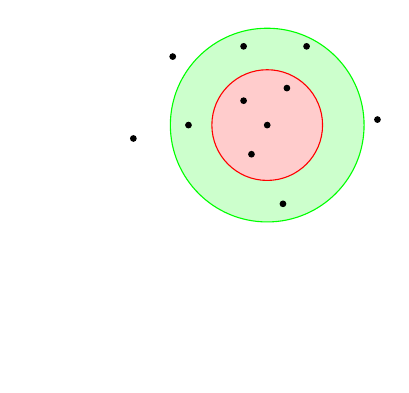
\begin{tikzpicture}
          \draw[white] (0,0) circle (1pt);
          \begin{scope}[shift={(3cm, 3cm)}]
            \draw[fill=green!20, draw=green] (0,0) circle (35pt);
            \filldraw[fill=red!20, draw=red] (0,0) circle (20pt);
            \filldraw[black] (0,0) circle (1pt);
            \filldraw[black] (0.5,1) circle (1pt);
            \filldraw[black] (-0.3,1) circle (1pt);
            \filldraw[black] (0.2,-1) circle (1pt);
            \filldraw[black] (-1,0) circle (1pt);
            \filldraw[black] (-0.3,0.31) circle (1pt);
            \filldraw[black] (0.25,0.47) circle (1pt);
            \filldraw[black] (-0.20,-0.37) circle (1pt);
            \filldraw[black] (-1.7,-0.17) circle (1pt);
            \filldraw[black] (-1.2,0.87) circle (1pt);
            \filldraw[black] (1.4,0.07) circle (1pt);
          \end{scope}
        \end{tikzpicture}
      \end{subfigure}%
      \begin{subfigure}{0.7\linewidth}
        \centering
        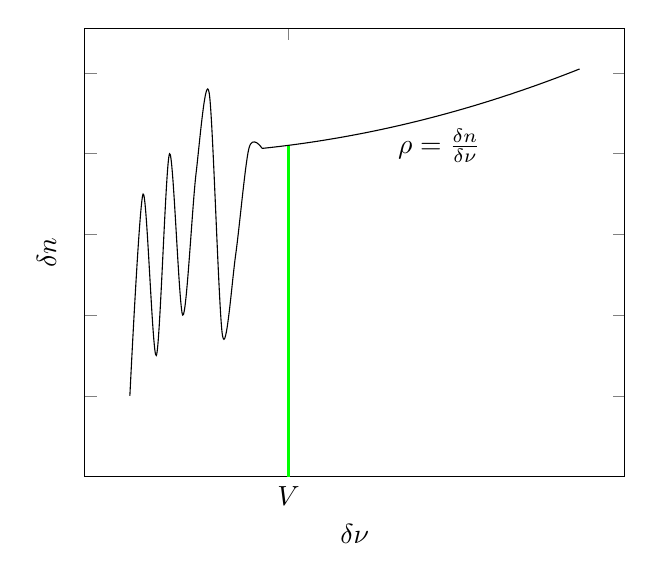
\begin{tikzpicture}
          \begin{axis}[
              xtick = {13},
              xticklabels = {$V$},
              yticklabels = {},
              ymin=0,
              xlabel = {$\delta \nu$},
              ylabel = {$\delta n$}
            ]
            \addplot[smooth] coordinates {
              (1, 2)
              (2, 7)
              (3, 3)
              (4, 8)
              (5, 4)
              (6, 7.5)
              (7, 9.5)
              (8, 3.5)
              (9, 5.5)
              (10, 8.132)
              (11, 8.132)
              % (12.5, 8.1)
              % (15, 8.3)
              % (17.5, 8.5)
              % (20, 9)
              % (30, 9.5)
            };
            \addplot [
              domain = 11:35,
              samples = 100
            ]
            {0.01 * (0.2 * x^2 - x + 800)};
            \addplot +[mark=none, color=green, thick] coordinates {(13, -1) (13, 8.2)};

          \end{axis}
            \node at (4.5, 4.2) {$\rho = \frac{\delta n}{\delta \nu}$};
        \end{tikzpicture}
      \end{subfigure}

    \end{center}
    \label{fig:0}
  \end{figure}


  Since matter is not continuous, we can't speak of a density at a point (in a mathematical sense) and
  thus, when we use the phrase ,,point'' we mean ,,at a point for homogeneous physical system''.

  We also introduce length scale separation % for 

  \begin{displaymath}
    \begin{matrix}
      \tm{molecular length scale} & \ll & \nu^{\frac{1}{3}} & \ll & L.
    \end{matrix}
  \end{displaymath}
  We call those characteristic length scales ,,\emph{micro}'', ,,\emph{muso}'' and ,,\emph{macro}'' respectively.
  

  \subsection{Equilibrium thermodynamics}
  \begin{figure}[H]
    \begin{subfigure}{0.5\linewidth}
      \centering
      \begin{tikzpicture}
        \node[anchor = south west] (image) at (0,0)
        {\includegraphics[width=\textwidth]{./images/00river.pdf}};
        \begin{scope}[x={(image.south east)}, y={(image.north west)}]
          \node at (0.35, 0.5) {$\vec u(\vec r, t)$};
          \node at (0.65, 0.5) {river};
          \draw [-stealth] (0.4,0.52) -- (0.5,.58);
        \end{scope}
      \end{tikzpicture}

    \end{subfigure}
    \begin{subfigure}{0.5\linewidth}
      \centering
      \begin{tikzpicture}
        \node[anchor=south west] (image) at (0,0)
        {\includegraphics[width=\textwidth]{./images/00ellipse.pdf}};
        \begin{scope}[x={(image.south east)}, y={(image.north west)}]
          \node at (0.3, 0.5) {$N, m$};
          \node at (0.43, 0.58) {$\vec u$};
          \draw [-stealth] (0.4,0.52) -- (0.5,.58);
        \end{scope}
      \end{tikzpicture}
    \end{subfigure}
  \end{figure}


  Let us examine an example of a water in a river.
  Assume that the water has some velocity $\vec {u}$, momentum $\vec{P}$ and also that it can 
  exchange mass and heat, the latter given by $\d Q = T \d S$.
  Therefore an incremental change in the energy of this system can be expressed as
  \begin{displaymath}
    \d E = \vec u \cdot \d \vec P - p \d V + T \d S + \mu \d N,
  \end{displaymath}
  where $\mu$ is the chemical potential of the system.
  Thus
  \begin{displaymath}
    E = E(\vec P, V, S, N).
  \end{displaymath}
  This is the \fndef{energy representation} of a thermodynamical system.
  Comparing the equations above we obtain
  \begin{displaymath}
    \d E = \underbrace{\ptf{E}{\vec P}}_{\vec u} \d \vec P + \underbrace{\ptf{E}{V}}_{- p} \d V 
    + \underbrace{\ptf{E}{S}}_{T} \d S + \underbrace{\ptf{E}{N}}_{\mu} \d N,
  \end{displaymath} % TODO add some explanation about the fact that \ptf{E}{\vec P} = \vec u.
  Those are called the Gibbs relation for $E$.

  If we want to compute it for a fixed entropy we get
  \begin{displaymath}
    \d S = \frac{1}{T} \d E - \frac{\vec u}{T} \d \vec P + \frac{p}{T} \d V - \frac{\mu}{T} \d N.
  \end{displaymath}
  Thus
  \begin{displaymath}
    S = S(E, \vec P, V, N), \quad
    \d S = \underbrace{\ptf{S}{E}}_{\frac{1}{T}} \d E + \underbrace{\ptf{S}{\vec P}}_{- \frac{\vec u}{T}} \d \vec P 
    + \underbrace{\ptf{S}{V}}_{\frac{p}{T}} \d V + \underbrace{\ptf{S}{N}}_{- \frac{\mu}{T}} \d N,
  \end{displaymath}
  Those are Gibbs relations for $S$.

  It is very tricky to control entropy --- it's much easier to control the temperature.
  To obtain a description of our system when $T$ is an independent variable we need to use another thermodynamical potential,
  % switch variables i.e. use other thermodynamical potential.
  which is Helmholz free energy.
  Transition is obtained by
  \begin{displaymath}
    (S \ra T) \quad F = E - TS, \quad F = F(\vec P, V, T, N)
  \end{displaymath}
  \begin{displaymath}
    \d F = - S \d T - p \d V  + \vec{u} \d \vec {P}  + \mu \d N.
  \end{displaymath}
  Now we can do the same to switch other variables. Thus we obtain
  \begin{displaymath}
    (V \ra P) \quad H = E + p V, \quad H = H(\vec P, p, S, N),
  \end{displaymath}
  which is called an enthalpy,
  \begin{displaymath}
    (S \ra T) \quad G = E + pV - TS, \quad G = G(\vec P, p , T, N),
  \end{displaymath}
  which is called a Gibbs potential.

  Now we want to consider if they are Galilean invariant
  % \todo Fig\#4.

  % \begin{figure}[ht]
  %   \centering
  %   \begin{tikzpicture}
  %     \node[anchor=south west] (image) at (0,0)
  %     {\includegraphics[width=0.5\textwidth]{./images/00splash.pdf}};
  %     \begin{scope}[x={(image.south east)}, y={(image.north west)}]
  %       \node at (0.3, 0.5) {$N, m$};
  %       \node at (0.43, 0.58) {$\vec u$};
  %       \draw [-stealth] (0.4,0.52) -- (0.5,.58);
  %     \end{scope}
  %   \end{tikzpicture}
  % \end{figure}

  \begin{displaymath}
    E(\vec P, V, S, N) = E_0 (V, S, N) + \frac{\vec P^2}{2 M},
  \end{displaymath}
  where $E_0$ is the \fndef{internal energy}.
  For other potentials we obtain
  \begin{displaymath}
    H(\vec P, p , S, N) = H_0(p, S, N) + \frac{\vec P^2}{2 M},
  \end{displaymath}
  \begin{displaymath}
    F(\vec P, V, T, N) = F_0(T, V, N) + \frac{\vec P^2}{2 M},
  \end{displaymath}
  \begin{displaymath}
    G(\vec P, V, T, N) = G_0(T, p, N) + \frac{\vec P^2}{2 M}.
  \end{displaymath}
  
  Using $\vec P = M \vec u$ we get
  \begin{displaymath}
    E = E_0 + \frac{1}{2} M \vec u ^2.
  \end{displaymath}
  \begin{displaymath}
    \d E = \d E_0 + \vec u \cdot \d \vec P,
  \end{displaymath}
  \begin{displaymath}
    \d S = - \frac{1}{T} \vec u \cdot \d \vec P + \frac{1}{T} \d E + \frac{p}{T} \d V - \frac{\mu}{T} \d N,
  \end{displaymath}
  \begin{displaymath}
    \d S = \frac{1}{T}\d E_0 + \frac{p}{T} \d V - \frac{\mu}{T} \d N 
    \qLRa S(\vec P , E , V, N) = S(E_0, V, N).
  \end{displaymath}
  Thus $S$ is a Galilean invariant.

  \subsection{Heterogenous macroscopic system}
  \todo Fig\#5

  \begin{figure}
    \centering
     \begin{tikzpicture}
       \node[anchor=south west] (image) at (0,0)
       {\includegraphics[width=0.25\textwidth]{./images/00Fig5.png}};
       \begin{scope}[x={(image.south east)}, y={(image.north west)}]
         \node at (0.6, 0.7) {$v = \d\vec r$}; % TODO what does it mean XD
         \node at (0.35, 0.15) {$\Omega$}; % TODO what does it mean XD
         \node at (0.95, 0.45) {$\mathbb{M} = \int_\Omega \rho(\vec r, t) \d \vec r$}; % TODO what does it mean XD
         \node at (0.95, 0.25) {$\mathbb{E} = \int_\Omega \epsilon(\vec r, t) \d \vec r$}; % TODO what does it mean XD
       \end{scope}
     \end{tikzpicture}
    \caption{Sample volume $\Omega$. $\rho$ stands for mass density, $\varepsilon$ for density of the system.}
    \label{fig:1.5}
  \end{figure}

  ,,Densities'' are extensive properties per unit volume.
  Assume that $V = \const$, $\d V = 0$.
  Example of densities
  \begin{itemize}
    \item $\rho = \frac{M}{V}$ mass density,
    \item $\vec j = \frac{\vec P}{V}$ momentum density,
    \item $\varepsilon = \frac{E}{V}$ energy density,
    \item $\sigma = \frac{S}{V}$ entropy density.
  \end{itemize}
  \begin{displaymath}
    \d E = \vec u \d \vec P - p \d V + T \d S + \mu \d N / \cdot \frac{1}{V}.
  \end{displaymath}
  \begin{displaymath}
    \d \varepsilon = \vec u \cdot \d \vec j + T \d \sigma + \mu\d n, \quad \d n = \frac{\d \rho}{m},
  \end{displaymath}
  \begin{displaymath}
    \rho = \frac{M}{V} = \frac{Nm}{V} = nm \qLRa \d n = \frac{\d \rho}{m}.
  \end{displaymath}
  Thus the energy fundamental representation in terms of densities can be written as
  \begin{displaymath}
    \varepsilon = \varepsilon(\vec j, \sigma, \rho).
  \end{displaymath}
  After performing a Galilean transform we get
  \begin{displaymath}
    \varepsilon(\vec j, \sigma, \rho) = \varepsilon_0(\sigma, \rho) + \frac{1}{2} \rho \vec u ^2.
  \end{displaymath}
  
  We can do the same to represent entropy in terms of densities
  \begin{displaymath}
    \d S = \dots \frac{1}{V} \qLRa  \d \sigma = \frac{1}{T} \d \varepsilon_0 - \frac{1}{T} \frac{\mu}{m} \d p.
  \end{displaymath}
  Thus
  \begin{displaymath}
    \sigma = \sigma(\varepsilon_0, \rho),
  \end{displaymath}
  which is also Galilean invariant.


  \subsection{Flow of Heterogenous macroscopic system}
  We are using thermodynamics equilibrium despite the fact that the system flows (which means that it is \emph{not} in the equilibrium).
  However there is no contradiction if we assume local, thermodynamical equilibrium.
  The same assumption is made in Navier-Stokes equations.

  From now one we use pseudostatic transition.
  The difference between quasi-static and pseudostatic is that pseudostatic need not to be reversible.
  Forces which acts during quasi-static transformation are those which keeps the system in equilibrium.
  Example of pseudostatic transition which is not quasi-static is a flow of viscose fluid.
  \todo Fig\#6.

  \begin{figure}
    \centering
     \begin{tikzpicture}
       \node[anchor=south west] (image) at (0,0)
       {\includegraphics[width=0.45\textwidth]{./images/00Fig6.png}};
       \begin{scope}[x={(image.south east)}, y={(image.north west)}]
         \node at (0.4, 0.9) {$\varepsilon(\vec j, \sigma, p)$}; 
         \node at (0.4, 0.75) {$\sigma(\varepsilon_0, p)$}; 
         \node at (0.2, 0.15) {$\Omega(t_1)$}; 
         \node at (0.6, 0.15) {$\Omega(t_2)$}; 
         \node at (0.9, 0.15) {$\Omega(t_3)$}; 
       \end{scope}
     \end{tikzpicture}
    \label{fig:1.6}
  \end{figure}
  
  
  \subsection{Kinematics}

  We have two descriptions: Eulerian and Lagrangian.
  Transition between them is obtained by
  % (\todo Fig\#7) 

  \begin{figure}
    \centering
     \begin{tikzpicture}
       \node[anchor=south west] (image) at (0,0)
       {\includegraphics[width=0.25\textwidth]{./images/00Fig7.png}};
       \begin{scope}[x={(image.south east)}, y={(image.north west)}]
         \node at (0.2, 0.1) {$\vec R$}; 
         \node at (0.9, 0.9) {$\vec r(\vec R, t)$}; 
       \end{scope}
     \end{tikzpicture}
    \label{fig:1.7}
  \end{figure}

  

  the solutions to the initial problem
  \begin{displaymath}
    \dfrac{\vec r}{t} = \vec u(r,t), \quad \vec r(t = 0) = \vec R.
  \end{displaymath}

  We want to find dependence of densities as the particle move, and those are
  \begin{center}
    \begin{tabular}{c|c|c|}
      & Euler & Lagrange \\
      \hline
      velocity & $\vec u(r, t) $ & $\vec u[ r(t), t]$\\
      density & $\rho(r, t)$ & $\vec \rho[ r(t), t]$\\
      \hline
    \end{tabular}
  \end{center}
  \begin{displaymath}
    \dfrac{\vec u}{t} = ?, \quad \dfrac{\rho}{t} = ?.
  \end{displaymath}
  
  To do that define $\beta = (\vec u, \rho, S, \sigma, \dots)$. 
  We want to find how $\beta$ change while following the motion 
  of the particle $r(t)$.
  \begin{displaymath}
    \dfrac{\beta}{t} = \dfrac{\beta[\vec r(t),t]}{t} = \ptf{\beta}{t} + \dfrac{r_1 }{t} \ptf{\beta}{r_1} 
    + \dfrac{r_2}{t} \ptf{\beta}{r_2} 
    + \dfrac{r_3}{t} \ptf{\beta}{r_3}  
  \end{displaymath}
  \begin{displaymath}
    = \ptf{\beta}{t} + \vec u (t)\cdot \nabla \beta 
    = \ptf{\beta}{t} + \d \beta(\vec u(t)).
  \end{displaymath}

  \begin{figure}
    \centering
     \begin{tikzpicture}
       \node[anchor=south west] (image) at (0,0)
       {\includegraphics[width=0.25\textwidth]{./images/00Fig8.png}};
       \begin{scope}[x={(image.south east)}, y={(image.north west)}]
         \node at (0.2, 0.1) {$\vec R$}; 
         \node at (0.7, 0.4) {$\beta(\vec r(t), t)$}; 
       \end{scope}
     \end{tikzpicture}
    \label{fig:1.8}
  \end{figure}


  Equation 
  \begin{equation}
    \dfrac{\beta}{t} = \ptf{\beta}{t} + \vec u(t) \cdot \nabla \beta,
    \label{eq:1}
  \end{equation}
  shows a relationship between Eulerian and Lagrangian world, because
  $\dfrac{\beta}{t}$ is a typical Lagrangian while fields (like $\vec u(t)$) are common in Euler's description.
  (Fields are Eulerian objects).
  We introduce a \fndef{total (material) derivative} as 
  \begin{displaymath}
    \dfrac{\dots}{t} = \underbrace{\ptf{\dots}{t}}_{\tm{local derivative}} + \underbrace{\vec u \cdot \nabla(\dots)}_{\tm{advective derivative}}.
  \end{displaymath}
  
  Acceleration of fluid particle
  \begin{displaymath}
    \beta = \vec u \qLRa \dfrac{\beta}{t} = \dfrac{\vec u}{t}.
  \end{displaymath}
  Consider converging chanell with a stationary flow, i.e. $\ptf{\vec u}{t} = 0$.

  % Fig\#9.

  \begin{figure}
    \centering
    \begin{tikzpicture}
      \node[anchor=south west] (image) at (0,0)
      {\includegraphics[width=0.25\textwidth]{images/00Fig9.png}};
        \begin{scope}[x={(image.south east)}, y={(image.north west)}]
        \node at (0.1, 0.6) {$\vec v_1$};
        \draw [-stealth] (0.1, 0.5) -- (0.2, 0.5);
        \node at (0.1, 0.3) {$r_1$};

        \node at (0.7, 0.6) {$\vec v_2$};
        \draw [-stealth] (0.7, 0.5) -- (0.9, 0.5);
        \node at (0.7, 0.3) {$r_2$};
        \end{scope}
    \end{tikzpicture}
    \label{fig:1.9}
  \end{figure}

  

  With that in mind
  \begin{displaymath}
    \dfrac{\vec u}{t} = \ptf{\vec u}{t} + \vec u \cdot \nabla \vec u = \vec u \cdot \nabla \vec u.
  \end{displaymath}
  The term $\vec u \cdot \nabla \vec u$ should be interpreted as follows.
  Treat $\vec u$ as a map $\vec u(\vec r): \RR^3 \ra \RR^3$. 
  Thus $\nabla \vec u$ is just a map $D \vec u: \RR^3 \ra \RR^3$ expressed by a matrix
  \begin{displaymath}
    \vec u(\vec r) = \begin{bmatrix}
      u_1 (r_1, r_2, r_3)\\
      u_2 (r_1, r_2, r_3)\\
      u_3 (r_1, r_2, r_3)
    \end{bmatrix}, \quad 
    D \vec u = \begin{bmatrix}
      \ptf{u_1}{r_1} & \ptf{u_1}{r_2} & \ptf{u_1}{r_3} \\
      \ptf{u_2}{r_1} & \ptf{u_2}{r_2} & \ptf{u_2}{r_3} \\
      \ptf{u_3}{r_1} & \ptf{u_3}{r_2} & \ptf{u_3}{r_3}
    \end{bmatrix}.
  \end{displaymath}
  Therefore inner product $\vec u \cdot \nabla \vec u$ really means
  \begin{displaymath}
    \vec u \cdot \nabla \vec u = (D \vec u)(\vec u).
  \end{displaymath}
  At least I think so\dots
  

  
  The term $\vec u \cdot \nabla \vec u$ is called a \fndef{convective acceleration}.
  Although the flow is stationary, the particle experiences acceleration related to movement along the flow lines. 
  
  
  We can interpret the fluid flow as a mapping which takes one point and maps it to the other.

  % Fig\#10.
  \begin{figure}
    \centering
    \begin{tikzpicture}
      \node[anchor=south west] (image) at (0,0)
      {\includegraphics[width=0.35\textwidth]{images/00Fig10.png}};
        \begin{scope}[x={(image.south east)}, y={(image.north west)}]
          \node at (0.3, 0.8) {$r(\cdot)$};
          \node at (0.6, 0.1) {$r^{-1}(\cdot)$};
        \end{scope}
    \end{tikzpicture}
    \label{fig:1.10}
  \end{figure}

  
  
  \paragraph{Streakline}

  \begin{figure}
    \centering
    \begin{tikzpicture}
      \node[anchor=south west] (image) at (0,0)
      {\includegraphics[width=0.25\textwidth]{images/00Fig11.png}};
        \begin{scope}[x={(image.south east)}, y={(image.north west)}]
          \node at (0.0, 0.2) {$\vec y$};
          \node at (0.8, 0.9) {$\vec r(\vec y, t)$};
        \end{scope}
    \end{tikzpicture}
    \caption{Streakline is a line made of all particles that for time $s$, $0 \leq s \leq t$ 
    passed through a fixed point $\vec y$.}
    \label{fig:1.11}
  \end{figure}

  

  Imagine a cigarette and assume that there is no diffusion. 
  The smoke is made out of small, fluid particles.
  The flow line is made out of fluid particles which were passing through $\vec y$ in the time interval
  $0 \leq s \leq t$.
  Suppose that we froze time at $t = t_0$.
  Choose point $A$.
  \fndef{Streakline} through the point $A$ is a curve made of all particles (in the given moment) that have passed
  through the point $A$ at some $t < t_0$.
  \begin{displaymath}
    \vec r [ \vec R(y,s), t], \quad 0 \leq s \leq t.
  \end{displaymath}

  \paragraph{Streamline}
  Streamline is a integral curve of a vector field $X(t)$ at a given time $t = t_0$.
  They do not intersect neither with each other nor with themselves.
  Equation:
  \begin{displaymath}
    \dfrac{r}{s} = \vec u(\vec r, t).
  \end{displaymath}

  \paragraph{Trajectory}
  \fndef{Trajectory} is a path traced by a chosen particle.

  For the stationary flow the streakline and streamline are the same.
  
  For stationary flows i.e. $(\ptf{u}{t} = 0)$.
  Trajectory $\equiv$ streakline $\equiv$ streamline.

  \section{Balance equations}
  $\vec u(\vec r, t)$ --- velocity field, $\rho(\vec r, t)$ --- density flow.
  They are not completely independent since the mass has to be conserved.
  % \todo Fig\#13

  \begin{figure}
    \centering
    \begin{tikzpicture}
      \node[anchor=south west] (image) at (0,0)
      {\includegraphics[width=0.35\textwidth]{images/00Fig12.png}};
    \end{tikzpicture}
    \caption{Streamline is just a flow of a vector field for at a fixed time $t$.}
    \label{fig:1.12}
  \end{figure}
  
  \begin{displaymath}
    M = \int_V \rho(\vec r, t) \d \vec r,
  \end{displaymath}
  \begin{displaymath}
    \ptf{M}{t} = \ptf{}{t} \in V \rho(\vec r, t) = \int_V \ptf{\rho(\vec r, t)}{t} \d \vec r.
  \end{displaymath}
  \begin{displaymath}
    \ptf{M}{t} = \int_V \ptf{\rho}{t} \d \vec r
    = -\int_{\partial V} \rho \vec u \cdot \vec n \d a,
  \end{displaymath}
  using Stokes theorem
  \begin{displaymath}
    = - \int_V \nabla \cdot (\rho \vec u)  \d \vec r.
  \end{displaymath}

  In other words
  \begin{displaymath}
    \int_V \left[ \ptf{\rho}{t} + \nabla \cdot (\rho \vec u) \right] \d \vec r = 0 ,
  \end{displaymath}
  and, since $V$ is arbitrary,
  \begin{displaymath}
    \ptf{\rho}{t} + \nabla \cdot (\rho \vec u) = 0.
  \end{displaymath}
  Which is called the \fnvi{continuity equation}.
  This is the general mass conservation, fluid can change density and so on.


  \chapter{Wykład 2}
  \section{Wektory styczne i kowektory}
  \paragraph{a)} Wektor styczny w punkcie to odwzorowanie
  \begin{displaymath}
    C^\infty(M) \ni f \mapsto v(f) \in \RR,
  \end{displaymath}
  spełniające
  \begin{itemize}
    \item liniowość $v(a f + b h) = a v(f) + b v(h)$, $\forall f,g \in C^\infty(M)$, $a,b \in \RR$
    \item Leinbniz $v(fh) = f(p) v(h) + v(f) h(p)$
  \end{itemize}

  \todo Fig1

  Pozostaje pytanie jak to wygląda w lokalnych mapach. 
  Rozważmy mapę $\varphi$ i różniczkowanie w punkcie $p \in U$, gdzie $U$ jest dziedziną mapy $\varphi$.
  Wtedy dla wektora stycznego $\vec v$:
  \begin{equation}
    \vec v: f \longmapsto \left( v^k \ptf{}{x^k} (f \circ \varphi^{-1}) \right) (x^1(p), \dots, x^n(p)).
  \end{equation}
  Co więcej, każdy wektor styczny daje się zapisać w tej postaci.
  Dodatkowo, jeśli mamy atlas to wszystkie wektory wyrażają się w ten sposób (to znaczy, że nie musimy szukać nowej mapy
  dla każdego z wektorów stycznych).

  Ogólnie. Jeśli $\vec v$ jest wektorem stycznym w $p \in M$ do $M$, a $M \supset U \os{\varphi}{\ra}\RR^n$
  to istnieją $v^1, \dots, v^n \in \RR$, takie, że $v(f)$ wyraża się poprzez
  \begin{displaymath}
    v(f) = \left(v^k \ptf{}{x^k } f\circ \varphi^{-1}\right) (\varphi(p)).
  \end{displaymath}
  \todo Fig2

  Zwyczajowo stosuje się notację uproszczoną
  \begin{displaymath}
    \vec v = v^k \ptf{}{x^k}
  \end{displaymath}
  ALE do tego musimy pamiętać, że to w lokalnym układzie współrzędnych.
  Ma to konsekwencje np. jak mamy ,,drugą'' pochodna tj. różniczkowanie raz po $x^i$, a raz po $y^i$, gdzie $x, y$ 
  to współrzędne w różnych mapach.
  
  Wektor styczny jest także związany z krzywymi na rozmaitości.
  Rozważmy krzywą $\gamma$ przechodzącą przez punkt $p$
  \begin{displaymath}
    \gamma : \tau \mapsto x^1(\tau), \dots, x^n(\tau), \quad (x^1(0), \dots, x^n(0)) = \varphi(p)
  \end{displaymath}
  
  \begin{displaymath}
    \dfrac{f \circ \varphi^{-1}}{\tau} ( x^1 (\tau), \dots, x^n(\tau)) 
    = \dfrac{x^i}{\tau} \ptf{}{x^i} (f \circ \varphi^{-1})|_{x(p)}
  \end{displaymath}

  Zauważmy, że różne funkcje mogą spełniać tę relację.
  Wniosek: wektor styczny w $P$ do $M$ to klasa równoważności krzywych takich, że
  \begin{displaymath}
    \dfrac{f(p(\tau))}{\tau}|_{\tau = 0} = \dfrac{f(q(\tau))}{\tau}|_{\tau = 0},
  \end{displaymath}
  oraz $p(0) = q(0)$.

  \todo Fig3

  \paragraph{c) Prawo transformacji}
  Żeby nie pisać cały czas
  \begin{displaymath}
    (y^1, \dots, y^n) = (\varphi' \cdot \varphi^{-1})(x^1, \dots, x^n), 
  \end{displaymath}
  gdzie $y^i$ to współrzędne w mapie $\varphi'$, a $x^i$ to współrzędne w mapie $\varphi$,
  będziemy pisać po prostu
  \begin{displaymath}
    y^k = y^k(x^1, \dots, x^n).
  \end{displaymath}

  Przy tej konwencji zamiana współrzędnych ma postać
  \begin{displaymath}
    v^i \ptf{}{x^i} = v^i\ptf{y^j}{x^i} \ptf{}{y^j} = \underbrace{ v^i \ptf{y^j}{x^i} }_{=: (v')^i}.
  \end{displaymath}
  
  Wniosek: jeśli $v = v^k \ptf{}{x^k} = (v')^l \ptf{}{(x')^l}$ to wtedy $(v')^l = \ptf{(x')^l}{x^k} v^k$.

  Przestrzeń wekorów stycznych do $M$ w punkcie $p \in M$ nazywamy \fndef{przestrzenią styczną} i oznaczamy 
  przez $T_pM$.

  \begin{lemma}
    $T_p M$ jest przestrzenią wektorową, czyli, jeśli $\vec v, \vec w \in T_pM$ to $ a\vec v + b \vec w \in T_pM$ 
    dla każdych $a, b\in \RR$.
  \end{lemma}

  Wniosek: Bazę w przestrzeni $T_pM$ tworzą wektory $\ptf{}{x^1}, \dots, \ptf{}{x^n}$ gdzie 
  $(x^1, \dots, x^n)$to dowolny układ współrzędnych.

  \paragraph{d) kowektory}
  Kowektorem jest element przestrzeni dualnej $T^*_p M$.
  
  \begin{example}
    Niech $f \in C^\infty(M)$, zdefiniujmy
    \begin{displaymath}
      T_p M \ni v \mapsto v(f) \in \RR.
    \end{displaymath}
    %, Łatwo sprawdzić, że $(av + bw)(f) = a v(f) + bw (f)$.
    Oznaczamy je $\d f $ i nazywamy \fndef{różniczką} funkcji $f$.
    Czyli $v\ctr \d f = v(f)$, tylko teraz patrzymy na to w ten sposób, że $f$ jest stałe, a $v$ się zmienia.
  \end{example}

  \begin{lemma}
    Dla każdego $\omega \in T_p^*M$ istnieją funkcje $f^1, \dots, f^n \in C^\infty(M)$ oraz współczynniki $\omega_1, \dots, \omega_n \in \RR$
    takie, że
    \begin{displaymath}
      \omega = \omega_i \d f^i.
    \end{displaymath}
  \end{lemma}

  Niech $(x^1, \dots, x^n)$ będzie układem współrzędnych. Rozważmy
  \begin{equation}
    \omega = \omega_i \d x^i.
    \label{eq:2.1}
  \end{equation}
  
  \begin{lemma}
    Wszystkie $\omega \in T^*M$ są postaci \ref{eq:2.1}.
  \end{lemma}
  \begin{proof}
    \begin{displaymath}
      v \ctr \omega = (v^k\ptf{}{x^k}) \ctr \omega 
      = v^k ( \ptf{}{x^k} \ctr \omega) 
      = \omega_k v^k 
      = (v^k \ptf{}{x^k}) \ctr(\omega_l \d x^l).
    \end{displaymath}
    
  \end{proof}

  \paragraph{Prawo transformacji}
  Przestrzenie dualne zawsze transformują się macierzą odwrotną.
  Explicit\'e wzór
  \begin{displaymath}
    \d x^k = \ptf{x^j}{x^k} \d (x')^k
  \end{displaymath}
  \begin{displaymath}
    (\omega')_k = \ptf{x^i}{(x')^k} \omega_i
  \end{displaymath}
  

  \section{Tensory}
  
  Rozważmy przestrzenie wektorowe $V, W$.
  Dla $v \in V$, $w\in W$ wprowadzamy
  \begin{displaymath}
    v \oitmes w.
  \end{displaymath}

  Rozważmy \fndef{formalnych kombinacji liniowych} elementów $(v, w) \in V \times W$.
  Są one postaci
  \begin{displaymath}
    a_1 ( v_1, w_1) +\dots + a_\mu(v_\mu, w_\mu), \quad \mu \in \NN.
  \end{displaymath}
  Zdefiniujmy relację równoważności 
  \begin{displaymath}
    (a v + b v', w) \sim a (v, w) + b (v', w)
  \end{displaymath}
  (analogicznie dla drugiej współrzędnej) oraz
  \begin{displaymath}
    (0, w) \sim (0, 0) \sim (v, 0).
  \end{displaymath}
  Iloczyn tensorowy przestrzeni $V, W$ definiuje się jako 
  \begin{displaymath}
    V \otimes W = \left\{ [(v, w)] = (v, w) / \sim | v\in V, w\in W \right\},
  \end{displaymath}
  gdzie $\sim$ jest zdefiniowaną wyżej relacją równoważności.

  Piszemy np.
  \begin{displaymath}
    v\otimes w = v^a w^b \ptf{}{x^a} \oitmes \ptf{}{x^b}, 
    \quad T = T^{ab} \ptf{}{x^a} \otimes \ptf{}{x^b}.
  \end{displaymath}

  \chapter{Wykład 3}
  \section{Tensorowe, formy różniczkowe, gęstości}
  \paragraph{Iloczyn tensorowy}
  Przykład
  \begin{displaymath}
    T^*_pM \otimes T^*_p M.
  \end{displaymath}
  Jest to przestrzeń odwzorowań biliniowych
  \begin{displaymath}
    T^*_pM \otimes T^*_p M \ni L : T_p M \times T_pM \ra \RR,
  \end{displaymath}
  \begin{displaymath}
    T_pM \otimes T_p M \ni L : T_p^*M \times T_p^*M \ra \RR,
  \end{displaymath}
  itp.

  Wprowadzamy oznaczenie
  \begin{displaymath}
    \bigwedge^N T^*_p M \subset (T^*_pM)^{\otimes n}.
  \end{displaymath}

  Formy różniczkowe są całkowicie antysymetryczne, czyli dla $\omega \in \bigwedge^N(T^*_p M)$ spełnia
  \begin{displaymath}
    \omega(v_1, \dots v_k, \dots, v_l \dots, v_n) = - 
    \omega(v_1, \dots v_l, \dots, v_k \dots, v_n).
  \end{displaymath}

  Własności
  \begin{enumerate}
    \item dla $N > \dim M$, $\bigwedge^N(T^*_pM) = \left\{ 0 \right\}$
    \item dla $N = \dim M$, $\dim \bigwedge^N(T^*_pM) = 1$.
  \end{enumerate}

  Niech $e^1, \dots, e^n \in T^*_pM$,
  \begin{displaymath}
    e^a \wedge e^b := e^a \otimes e^b - e^b \otimes e^a,
  \end{displaymath}
  a dla 
  \begin{displaymath}
    e^{a_1} \wedge \dots \wedge e^{a_l} = \sum_\sigma (-1)^{\tm{sgn} \sigma} e^{a_{\sigma(1)} \otimes\dots \otimes e^{a_{\sigma(l)}}.
  \end{displaymath}

  Matematyczny zapis
  \begin{displaymath}
    \bigwedge^k T^*_pM \ni \omega = \omega_{a_1,\dots,a_k} e^{a_1}\otimes \dots \otimes e^{e_k} 
    = \frac{1}{k!}\omega_{a_1,\dots,a_k} e^{a_1}\wedge \dots \wedge e^{e_k} .
  \end{displaymath}

  Zapis fizyczny dla $\alpha \in \bigwedge^kT^*M, \beta \in \bigwedge^lT^*M$ mamy
  \begin{displaymath}
    \alpha \wedge \beta = \left( \frac{1}{k!} \alpha_{a_1,\dots, a_k} e^{a_1} \wedge \dots \wedge e^{a_n} \right)
    \wedge \left( \frac{1}{l!} \beta{b_1,\dots, b_l} e^{b_1} \wedge \dots \wedge e^{b_l} \right)
  \end{displaymath}
  \begin{displaymath}
    = \frac{1}{k!}\frac{1}{l!} \alpha_{a_1,\dots, a_k}\beta{b_1,\dots, b_l} e^{a_1} \wedge \dots \wedge e^{a_n} 
    \wedge    e^{a_1} \wedge \dots \wedge e^{b_l} 
  \end{displaymath}

  Mamy także iloczyn wewnętrzny, zwany też zwężeniem lub kontrakcją:
  \begin{displaymath}
    v \ctr \omega = \frac{1}{(k - 1)!} v^{a_1} \omega_{a_1, \dots, a_k} e^{a_2} \wedge \dots \wedge e^{a_k}.
  \end{displaymath}
  Własność:
  \begin{displaymath}
    v \ctr (\alpha \wedge \beta) = (v \ctr \alpha) \wedge \beta + (-1)^k \alpha \wedge (v \ctr \beta).
  \end{displaymath}
  
  \section{Gęstości}
  Rozpocznijmy od rozważenia symbolu Levi-Civity.
  Zauważmy, że nie jest on tensorem. Jeśli by był to znaczy, że transformowałby się jak tensor, 
  a tego nie robi (mnoży się razy $\det A$) gdzie $A \in GL(M)$.
  W fizyce tego nie widać, bo stosujemy transformacje z $SL(M)$, czyli ten wyznacznik daje 1.

  Jest ważne żeby nie trakotować formy maksymalnego wymiaru jako funkcji --- wynika to stąd, że nie 
  jest ona niezmiennicza przy zamianie współrzędnych.
  Obiekt który przy zamianie współrzędnych z $\left\{e^i\right\}$ na $\left\{ f^i \right\}$ 
  transformuje się jak
  \begin{displaymath}
    f(p) \mapsto \det A(p) f(p)
  \end{displaymath}
  nazywamy \fndef{pseudogęstością}. 
  Jeśli w powyższym wzorze damy $\abs{\det A}$ zamiast $\det A$ to 
  dostaniemy \fndef{gęstość}. 
  Żeby być całkowicie poprawnym to 
  \begin{definition}
    Niech $p \in M$ będzie punktem rozmaitości, a $\mathfrak{b}$ będzie dowolną bazą w przestrzeni stycznej.
    Odwzorowanie które parze $(p, \mathfrak{b})$ przyporządkowuje liczbę z $\RR$, a po zmianie współrzędnych
    transformuje sią jak 
    \begin{displaymath}
      \rho (p, A \mf{b}) = \abs{\det A}^\alpha \rho(p, \mf{b})
    \end{displaymath}
    nazywamy \fndef{$\alpha$-gęstością}.
  \end{definition}
  
  \section{Pola tensorowe i operacje}
  \paragraph{a) Pole wektorowe}
  \fndef{Polem wektorowym} na rozmaitości różniczkowej $M$ nazywamy gładkie odwzorowanie 
  \begin{displaymath}
    M \ni p \mapsto v \in T_p M,
  \end{displaymath}
  jeśli odwzorowanie to jest gładkie.
  Gładkość oznacza, że w lokalnym układzie współrzędnych, w którym $TM|_U$ można zapisać jako
  $U \times \RR^n$ odwzorowanie
  \begin{displaymath}
    U \ni p \mapsto v  \in \RR^n
  \end{displaymath}
  jest gładkie.
  W lokalnym układzie współrzędnych pola wektorowe można zapisywać jako
  \begin{displaymath}
    v = v^a \ptf{}{x^a}.
  \end{displaymath}
  Dodatkowo mamy nawias pól wektorowych dany poprzez
  \begin{displaymath}
    [v, w] (f) = v(w(f)) - w(v(f)),
  \end{displaymath}
  a w układzie współrzędnych
  \begin{displaymath}
    [v, w] = \left( v^a \ptf{w^b}{x^a} - w^a \ptf{v^b}{x^a} \right) \ptf{}{x^b}.
  \end{displaymath}
  
  
  \paragraph{Pola tensorowe}
  Każde pole tensorowe można wyrazić przy pomocy iloczynów tensorowych (i ich kombinacji liniowych) pól wektorowy i jednoform.

  \paragraph{Pochodna Liego pola wektorowego}
  Niech $v, w \in \XX(M)$. Wówczas \fndef{pochodną Liego} pola wektorowego $w$ w kierunku pola $v$ nazywamy
  \begin{displaymath}
    \ld_v w :=[v, w].
  \end{displaymath}
  Niech $f \in C^\infty(M)$. 
  Wówczas pochodną Liego funkcji $f$ w kierunku pola $v$ nazywamy
  \begin{displaymath}
    \ld_v f:= v(f).
  \end{displaymath}
  Podobnie
  \begin{displaymath}
    \ld_v(\d f) := \d (\ld_v f).
  \end{displaymath}

  Dodatkowo wymagamy, żeby pochodna Liego spełniała regułę Leibniza
  \begin{displaymath}
    \ld_v(v_1\otimes \dots \otimes v_k \otimes \omega_1\otimes\dots \otimes \omega_l) = 
    (\ld_v(v_1))\otimes \dots \otimes v_k \otimes \omega_1\otimes \dots \otimes\omega_l + \dots.
  \end{displaymath}
  Z tego już wynika działanie pochodnej Liego na dowolne pole wektorowe.


  \paragraph{Przykład} 
  Niech 
  \begin{displaymath}
    L = L_{ab} \d x^a \otimes \d x^b, \quad v = v^a \ptf{}{x^a}.
  \end{displaymath}
  Wtedy 
  \begin{displaymath}
    \ld_vL = \ld_v(L_{ab} \d x^a \otimes \d x^b) = v(L_{ab}) \d x^a \otimes \d x^b 
    + L_{ab} (\d v(x^a)) \otimes \d x^b
    + L_{ab} \d x^a\otimes v(x^b)
  \end{displaymath}
  \begin{displaymath}
    = v(L_{ab}) \d x^a \otimes \d x^b  
    + L_{ab} \ptf{v^a}{x^c}\d x^c \otimes \d x^b
    + L_{ab} \ptf{v^b}{x^c}\d x^a \otimes \d x^c.
  \end{displaymath}
  
  
  \paragraph{Przykład 2}
  \begin{displaymath}
    \ld_v \ptf{}{x^b} = - \ptf{v^a}{x^b}\ptf{}{x^a}.
  \end{displaymath}

  \begin{lemma}
    \begin{displaymath}
      \ld_v(w^a \alpha_a) = (\ld_v w)^a\alpha_a + w^a (\ld_v\alpha)_a.
    \end{displaymath}
    
  \end{lemma}

  \chapter{Wykład 4}

  Rozkład jazdy
  \begin{enumerate}
    \item Pochodna Liego
    \item Pochodna zewnętrzna
    \item Związki pomiędzy $\ld_\xi$ oraz $\d$
    \item Całka z $k$-formy
    \item Uwagi: $T(M)$, $T^*(M)$ jako rozmatiości
      \begin{enumerate}
        \item wiązki naturalne
        \item wiązki stowarzyszone
        \item wiązki główne
      \end{enumerate}
    \item 
  \end{enumerate}

  
  \section{Pochoda zewnętrzna}

  Wprowadźmy oznaczenia 
  \begin{itemize}
    \item $\Gamma(T^*M)$ --- przestrzeń pól kowektorowych
    \item $\Gamma(\gibwedge^k(T^*M))$ --- przestrzeń pól $k$-form różniczkowych
  \end{itemize}
  Różniczka zewnętrzna
  \begin{displaymath}
    \d : \Gamma(\bigwedge^k T^*M) \ra \Gamma(\bigwedge^{k - 1}T^*M),
  \end{displaymath}
  z własnościami
  \begin{align*}
    \d (\alpha \wedge \beta) = \d \alpha \wedge \beta + (-1)^k \alpha \wedge\d \beta \\
    \d (\alpha + \beta) = \d \alpha + \d \beta\\
    \d^2 = 0
  \end{align*}

  \section{Związki pomiędzy $\ld$ a $\d$}
  Niech $\omega \in \Gamma(\bigwedge^k T^*M)$, $\xi \in \Gamma(TM)$
  \begin{displaymath}
    \ld_\xi \omega = \xi \ctr \d \omega + \d (\xi \ctr \omega)
  \end{displaymath}

  Geometryczny wzór na nawias Liego
  \begin{displaymath}
    \d \omega(v, w) = v(w \ctr \omega) - w(v \ctr \omega) - [v,w]\ctr\omega.
  \end{displaymath}
  

  Przykład liczenia pochodnej Liego na tensorach
  \begin{displaymath}
    \ld_V T_{ab} \d x^a \otimes \d x^b = v(T_{ab}) + T_{cb} \ptf{v^c}{x^a}+ T_{ca} \ptf{v^c}{x^b},
  \end{displaymath}
  \begin{displaymath}
    \ld_V T^{ab}\ptf{}{x^a} \otimes \ptf{}{x^b} = v(T^{ab}) - T^{cb} \ptf{v^c}{x^a} - T_{ca} \ptf{v^c}{x^b},
  \end{displaymath}

  \section{Całki z form różniczkowych}
  
  Rozważmy rozmaitość $M$ i formę $\omega \in \Omega^n$.
  Dodatkowo załóżmy, że $\supp\omega \n \chi_I(U_I)$ dla pewnej lokalnej mapy.
  Definiujemy 
  \begin{displaymath}
    \int_M\omega = \int_{U_I} \omega  = \int \omega_{1, \dots, n} \d x^1 \wedge \dots \wedge \d x^n.
  \end{displaymath}
  Przy orientacji kluczowa jest orientacja na $M$.
  Jeśli mamy dwie mapy, $(U_I, \chi_I)$, oraz $(U_J, \chi_J)$ ze współrzędnymi odpowiednio $x^1, \dots, x^n$
  oraz $y^1, \dots, y^n$ to nazywamy je \fndef{zgodnie zorientowanymi} jeśli 
  \begin{displaymath}
    \forall a, b \quad \det \left( \ptf{x^a}{y^b} \right) > 0,
  \end{displaymath}
  na przecięciu $U_I\cap U_J$.
  Rozmatiość nazywamy \fndef{zorientowaną} jeśli można na niej zadać atlas w którym każde dwie mapy mają zgodną
  orientację.
  Całkować można tylko na rozmaitościach zorientowanych.
  Wynika to z tego, że przy zmianie bazy pod całką wyskakuje znak --- jeśli rozmaitość jest zorientowana to 
  nie ma problemu, bo ten znak jest zawze taki sam.

  Jeśli chcemy całkować na rozmaitości niespójnej to powinniśmy zdefiniować rozkład jedności.
  Zakłądamy, że istnieje rozkłąd jedności, czyli zbiór funkcji $\phi_\chi$ takich, że
  \begin{displaymath}
    \forall p \in M, \phi_\chi \neq 0 \tm{dla skończonego pozbioru zbioru }\chi
  \end{displaymath}
  oraz
  
  
  \chapter{Wykład 6}
  \paragraph{Koneksja}
  Koneksja na $TM$. 
  Jeśli dany jest reper $e^1, \dots, e^n$ to macierz koneksji wyraza się przez $\Gamma^i_j$, $i, j = 1\dots, n$,
  \begin{displaymath}
    e^{ij} = (a^{-1})^i_j e^j, \quad (\Gamma')^i_j = (a^{-1})^i_k \Gamma^k + (a^{-1})^i_k \d a^k_j.
  \end{displaymath}

  
  \paragraph{Krzywizna}
  Krzywizna
  \begin{displaymath}
    \mc{R}^i_j = \d \Gamma^i_j + \Gamma^i_k \wedge \Gamma^k_j = \frac{1}{2} R^i_{jkl} e^k \wedge e^l.
  \end{displaymath}
  Przy zmianie repera na $(e')^i = (a^{-1})^i_k e^k$ $\mv{R}$ zmienia się na
  \begin{displaymath}
    (\mv{R}')^i_j = (a^{-1})^i_k \mc R^k_l a^l.
  \end{displaymath}

  Podsumowując
  \begin{displaymath}
    \Gamma' = a^{-1} \Gamma a + a^{-1} \d a, \quad \mc{R}' = a^{-1} \mc{R} a.
  \end{displaymath}

  \paragraph{Pochodna kowariantna}
  Pomyślmy teraz o polu wektorowym jak o funkcji o wartościach wektorowych.
  Mamy wtedy następujący wzór
  \begin{displaymath}
    D v^i = \d v^i + \Gamma^i_j v^j.
  \end{displaymath}

  Dla k-formy mamy
  \begin{displaymath}
    D \omega^i = \d \omega^i + \Gamma^i_j \wedge \omega^j.
  \end{displaymath}

  \begin{lemma}
    Druga pochodna kowariantna dla współrzędnej
    \begin{displaymath}
      D^2\omega^i = R^i_j \wedge\omega^j.
    \end{displaymath}
  \end{lemma}
  Dla funkcji mamy $D \omega = \d \omega$.

  \paragraph{Różniczka kowarianta formy o wartościach kowektorowych}
  Niech $\omega$ będzie jednoformą, $\omega = \omega_i e^i$.
  Patrzymy na to jak na zeroformę o wartościach w $T^*_xM$.
  Pochodną kowariantna dla jednoformy jest równa
  \begin{displaymath}
    D \omega_i = \d \omega_i - \Gamma^j_i \omega_j.
  \end{displaymath}

  Wytłumaczenie dlaczego powinien być ten minus: rozważmy $v^i\omega_i$ i policzmy 
  $\d (v^i\omega_i) = (\d v^i)\omega_i + v^i \d \omega_i$.
  Licząc dalej dostajemy
  \begin{displaymath}
    D(v^i\omega_i) \os{?}{=} (Dv^i)\omega_i + v^i (D\omega_j).
  \end{displaymath}
  Żeby równość zachodziła bierzemy minus, wtedy się rzeczy skracają.
  
  \begin{displaymath}
    D \omega^{ij} = \d \omega^{ij} + \Gamma^i_l \wedge \omega^{lj} - \Gamma^j_l \wedge\omega^{il}.
  \end{displaymath}
  $D$ jest przemienne ze zwężaniem indeksów.
  
  \paragraph{Przykład}
  Sprawdźmy jak to działa na deltę Kroneckera.
  \begin{displaymath}
    D \delta^i_j = \d \delta^i_j + \Gamma^i_l \delta^l_j - \Gamma^k_j \delta^i_k.
  \end{displaymath}

  \paragraph{Przykład 2}
  Niech $\omega^i = \omega^i_j e^j = \delta^i_j e^j = e^i$
  \begin{displaymath}
    De^i = \d e^i \Gamma^i_j \wedge e^j = T^i = \frac{1}{2} T^i_{jk} e^j\wedge e^k.
  \end{displaymath}
  Dla repera holonomicznego mamy (MOŻE BYĆ BŁĄD)
  \begin{displaymath}
    D(\d x^i) = \d (\d x^i) + \Gamma^i_j \wedge \d x^i = \Gamma^i_{jk} \d x^k \wedge \d x&j 
    = \frac{1}{2} \left( \Gamma^i_{jk} - \Gamma^i_{kj} \right) \d x^k \wedge \d x^j.
  \end{displaymath}
  
  \paragraph{Pochodna kowariantna}
  Niech $T^i_j$ będzie polem tensorowym (0 formą o wartościach tensorowych).
  Wtedy różniczkę kowariantną nazywamy z definicji \fndef{pochodną kowariantną}
  \begin{displaymath}
    \nabla T^{i\dots}_{j\dots} = D T^{i \dots}_{j\dots}
  \end{displaymath}
  \begin{displaymath}
    \nabla_k T^{i\dots}_{j\dots} e^k\otimes e_i\otimes \dots \otimes e^j \dots
  \end{displaymath}
  
  
  \begin{displaymath}
    \nabla_v = \nabla_i v^j e^i\otimes e_j
  \end{displaymath}
  
  


  
  
  
  

  
  
  
  

  

  
  

  
  
\end{document}
